
\documentclass[submit]{harvardml}

% Put in your full name and email address.
\name{Matthew Leifer}
\email{matthewleifer@college.harvard.edu}

% List any people you worked with.
\collaborators{%
  John Doe,
  Fred Doe
}

% You don't need to change these.
\course{CS181-S17}
\assignment{Assignment \#3}
\duedate{5:00pm March 24, 2016}

\usepackage[OT1]{fontenc}
\usepackage[colorlinks,citecolor=blue,urlcolor=blue]{hyperref}
%\usepackage[pdftex]{graphicx}
\usepackage{subfig}
\usepackage{fullpage}
\usepackage{amsmath}
\usepackage{amssymb}
\usepackage{color}
\usepackage{todonotes}
\usepackage{listings}
\usepackage{common}
\usepackage{bm}

\usepackage[mmddyyyy,hhmmss]{datetime}

\definecolor{verbgray}{gray}{0.9}

\lstnewenvironment{csv}{%
  \lstset{backgroundcolor=\color{verbgray},
  frame=single,
  framerule=0pt,
  basicstyle=\ttfamily,
  columns=fullflexible}}{}

\begin{document}
\begin{center}
{\Large Homework 3: Max-Margin and SVM}\\
\end{center}
\subsection*{Introduction}

This homework assignment will have you work with max-margin methods
and SVM classification. The aim of the assignment is (1) to further
develop your geometrical intuition behind margin-based classification
and decision boundaries, (2) to explore the properties of kernels and
how they provide a different form of feature development from
basis functions, and finally (3) to implement a basic Kernel based
classifier.

There is a mathematical component and a programming component to this
homework.  Please submit your PDF and Python files to Canvas, and push
all of your work to your GitHub repository. If a question requires you
to make any plots, like Problem 3, please include those in the
writeup.

\newpage
%%%%%%%%%%%%%%%%%%%%%%%%%%%%%%%%%%%%%%%%%%%%%
% Problem 1
%%%%%%%%%%%%%%%%%%%%%%%%%%%%%%%%%%%%%%%%%%%%%
\begin{problem}[Fitting an SVM by hand, 7pts]
  For this problem you will solve an SVM without the help of a
  computer, relying instead on principled rules and properties of
  these classifiers.

Consider a dataset with the following 7 data points each with $x \in \reals$ : \[\{(x_i, y_i)\}_i =\{(-3
, +1 ), (-2 , +1 ) , (-1,  -1 ), (0, -1), ( 1 , -1 ), ( 2 , +1 ), ( 3 , +1 )\}\] Consider
mapping these points to $2$ dimensions using the feature vector $\bphi(x) =  (x, x^2)$. The hard margin classifier training problem is:
%
\begin{align}
  &\min_{\mathbf{w}, w_0} \|\mathbf{w}\|_2^2 \label{eq:dcp} \\
  \quad \text{s.t.} \quad & y_i(\mathbf{w}^\top \bphi(x_i) + w_0) \geq 1,~\forall i \in \{1,\ldots, n\}\notag
\end{align}

The exercise has been broken down into a series of questions, each
providing a part of the solution. Make sure to follow the logical structure of
the exercise when composing your answer and to justify each step.

\begin{enumerate}
\item Plot the training data in $\reals^2$ and draw the decision boundary
of the max margin classifer.
%
\item  What is the value of the margin achieved by the optimal
decision boundary? 
%
\item What is a vector that is orthogonal to the decision boundary?

%
\item Considering discriminant $h(\bphi(x);\boldw,w_0)=\boldw^\top\bphi(x) +w_0$, 
give an expression for {\em all possible} $(\boldw,w_0)$ that define
the optimal decision boundary. Justify your answer.

%
%dcp: answer is $a x^2-b=0$, $a>0$, $b/a=5/2$.
%


  \item Consider now the training problem~\eqref{eq:dcp}. Using
your answers so far, what particular solution
to $\boldw$ will be optimal for this optimization
problem?
%%
%

  \item Now solve for
the corresponding value of $w_0$, using your general expression 
from part~(4.) for the optimal decision boundary.
Write down the discriminant
function $h(\bphi(x);\boldw,w_0)$.


\item What are the support
vectors of the classifier?
 Confirm that the solution in part~(6.) makes the constraints in~\eqref{eq:dcp} binding
for support vectors.

\end{enumerate}

\end{problem}
\subsection*{Solution}
\begin{enumerate}
	\item  This is the graph of the transformed $x$'s.  The margin boundary corresponds to $y = 2.5$.  \\ \includegraphics[width=0.5\textwidth]{Question_1_Graph.eps}
	
	\item The margin is 1.5. \\
	
	\item Because the decision boundary corresponds to $y = 2.5$, an orthogonal vector is $[0,1]$ \\
	
	\item By definition, the value of the discriminant function for a point on the decision boundary must be 0.  So, $h(\phi(x); \boldw, w_0) = \boldw^T\phi(x) + w_0 = [0, C] \cdot [\sqrt{2.5}, 2.5]^T + w_0 = 0$ \\
	$2.5c + w_0 = 0$ \\
	$w_0 = -2.5c$ \\
	So, $(\boldw, w_0) = ([0, C], -2.5C)$ \\
	
	\item  The optimal form of $\boldw$ is the one such that the constraint in equation (1) is binding.  Thereofre, the $C$ that optimized it is the one that makes that constraint equal to 1 for the $x$'s on the margin and that the value of the discriminant is as small as possible without making any of the (correctly classified) data points less than 1 away from the margin.  Those are (-1,1), (1,1), (-2, 4), and (2, 4). \\
	So, for $(\pm 2, 4)$,  $1(4C - 2.5C) = 1$, which means $C = \frac{2}{3}$ and for $(\pm 1, 1)$, $-1(C - 2.5C) = 1$, which means $C = \frac{2}{3}$ \\\\
	
	\noindent $\boldw = [0, \frac{2}{3}]$
	
	\item Because $w_0 = -2.5C$ and $C = \frac{2}{3}$, $w_0 = -\frac{5}{3}$ \\
	$h(x; \boldw, w_0) = \frac{2}{3}x^2 - \frac{5}{3}$ 
	
	\item The support vectors are $x = \pm 1, \pm 2$, which as show in (4) make sthe constraint binding.  
	
	
\end{enumerate}



\newpage
%%%%%%%%%%%%%%%%%%%%%%%%%%%%%%%%%%%%%%%%%%%%%
% Problem 2
%%%%%%%%%%%%%%%%%%%%%%%%%%%%%%%%%%%%%%%%%%%%%
\begin{problem}[Composing Kernel Functions, 10pts]


  A key benefit of SVM training is the ability to use kernel functions
  $K(\boldx, \boldx')$ as opposed to explicit basis functions
  $\bphi(\boldx)$. Kernels make it possible to implicitly express
  large or even infinite dimensional basis features. We do this 
  by computing $\bphi(\boldx)^\top\bphi(\boldx')$ directly, without ever computing $\bphi(\boldx)$ .

  When training SVMs, we begin by computing the kernel matrix $\boldK$,
  over our training data $\{\boldx_1, \ldots, \boldx_n\}$.  The kernel
  matrix, defined as $K_{i, i'} = K(\boldx_i, \boldx_{i'})$, expresses
  the kernel function applied between all pairs of training points.

  In class, we saw Mercer's theorem, which tells us that any function
  $K$ that yields a positive semi-definite kernel matrix forms a valid
  kernel, i.e. corresponds to a matrix of dot-products under
  \textit{some} basis $\bphi$. Therefore instead of using an explicit
  basis, we can build kernel functions directly that fulfill this
  property.

  A particularly nice benefit of this theorem is that it allows us to
  build more expressive kernels by composition.  In this problem, you
  are tasked with using Mercer's theorem and the definition of a
  kernel matrix to prove that the following  compositions are valid kernels, 
  assuming $K^{(1)}$ and $K^{(2)}$ are valid kernels. Recall that a positive semi-definite matrix $\boldK$ requires $\mathbf{z}^\top \mathbf{Kz} \geq 0,\ \forall\ \mathbf{z} \in \reals^n$.

  \begin{enumerate}
  \item $K(\boldx, \boldx') = c\,K^{(1)}(\boldx, \boldx') \quad \text{for $c>0$}$
  \item $ 	K(\boldx, \boldx')= K^{(1)}(\boldx, \boldx') + K^{(2)}(\boldx, \boldx')$
  \item   $ K(\boldx, \boldx') = f(\boldx)\,K^{(1)}(\boldx, \boldx')\,f(\boldx') \quad
  \text{where $f$ is any function from~$\reals^m$ to $\reals$}$
  \item $ K(\boldx, \boldx') = K^{(1)}(\boldx, \boldx')\,K^{(2)}(\boldx,
  \boldx')$

  [Hint: Use the property that for any
  $\bphi(\boldx)$,
  $K(\boldx, \boldx') = \bphi(\boldx)^\top\bphi(\boldx')$ forms a
  positive semi-definite kernel matrix. ]
  \item 
  \begin{enumerate}
  	\item The $\exp$ function can be written as,
  	$$\exp(x) = \lim_{i\rightarrow \infty} \left(1 + x + \cdots + \frac{x^i}{i!}\right).$$
  	  Use this to show that $\exp(xx')$ (here
          $x, x'\in \reals$)) can be written as $\bphi(x)^\top \bphi(x')$ for some basis function $\bphi(x)$. Derive this basis function,
          and explain why this  would be hard to use as a basis in standard logistic regression.
  	\item Using the previous identities, show that $K(\boldx, \boldx') = \exp( K^{(1)}(\boldx, \boldx'))$ is a valid kernel.
  	

  \end{enumerate}
  \item  Finally use this analysis and previous identities to prove the validity of the Gaussian kernel:
  \begin{align*}
	K(\boldx, \boldx') &= \exp \left( \frac{-||\boldx - \boldx'||^2_2}{2\sigma^2} \right) 
  \end{align*}
  \end{enumerate}



 \end{problem}
\subsection*{Solution}
\begin{enumerate}
	\item $K(\boldx, \boldx') = cK^{(1)}(\boldx,\boldx')$ for $c > 0$ \\
	$\boldz^TK\boldz = \boldz^TcK\boldz = c(\boldz^TK^(1)\boldz)$ and because $c$ is greater than zero and $K^{(1)}$ is a valid kernel matrix $c(\boldz^TK^{(1)}\boldz)$ is always greater than 0 and so this is a valid kernel.  \\
	
	\item $K(x, x') = K^{(1)}(\boldx,\boldx') + K^{(2)}(\boldx,\boldx')$ \\
	$\boldz^TKz = \boldz^T(K^{(1)} + K ^{(2)})\boldz = \boldz^TK^{(1)}\boldz + \boldz^TK^{(2)}\boldz$ and because $K^{(1)}$ and $K^{(2)}$ are both valid kernel functions then $\boldz^TK^{(1)}\boldz + \boldz^TK^{(2)}\boldz$ is always greater than zero and so $K$ is also a valid kernel. 
	
	\item $K(\boldx, \boldx') = f(\boldx)K^{(1)}f(\boldx')$, which can be rewritten as $f(\boldx)\phi(\boldx)^T\phi(\boldx')f(\boldx')$ per Mercer's theorem.  Then, using the hint in part 4, this can be rewritten as $g(\boldx)^Tg(\boldx')$ where $g(\boldx) = f(\boldx)\phi(\boldx)$ which is a valid kernel. 
	
	\item $K(\boldx, \boldx') = K^{(1)}(\boldx, \boldx')K^{(2)}(\boldx, \boldx') \\\\
	= \bphi_1(\boldx)^T\bphi_1(\boldx')\bphi_2(\boldx)^T\bphi_2(\boldx') \\\\
	= \displaystyle\sum_{i = 1}^{N}\phi_{1i}(x)\phi_{1i}(x') \cdot \displaystyle\sum_{j = 1}^{M}\phi_{2j}(x)\phi_{2j}(x') \\\\
	= \displaystyle\sum_{i = 1}^{N}\displaystyle\sum_{j = 1}^{M} \phi_{1i}(x)\phi_{2j}(x)\phi_{1i}(x')\phi_{2j}(x') $ \\\\
	and so we can construct a new function $\phi_3$ such that this sum equals\\
	$\displaystyle\sum_{k = 1}^{MN}\phi_{3k}(x)\phi_{3k}(x') \\ 
	= \bphi_3(x)^T\bphi_3(x')$, which is indeed a valid kernel.  
	\item 
	\begin{enumerate}
		\item The Taylor series for $\textup{exp}(x,x') = \displaystyle\sum_{i = 0}^{\infty}\dfrac{(xx')^i}{i!}$.  Therefore, if we define $\phi: \reals \to \reals^{\infty}$ such that $\phi(x) = [1 x \frac{x^2}{\sqrt{2!}} ... \frac{x^n}{\sqrt{n!}}]^T$ and so when we take $\phi(x)^T\cdot \phi(x')$ we recover the Taylor series for $\textup{exp}(x,x')$. Because this is an infinite dimensional basis function, it would be hard to use in logistic regression.   
		
		\item $K(\boldx, \boldx') \\\\ 
		= \textup{exp}(K^{1}(\boldx, \boldx'))  \\\\
		= \displaystyle\sum_{i = 0}^{\infty}\dfrac{K^{(1)}(\boldx, \boldx')^i}{i!} \\\\
		= \displaystyle\sum_{i = 0}^{\infty}\dfrac{(\phi(x)^T\phi(x'))^i}{i!}$ \\\\
		By part (4), we know that $K^{(1)}(\boldx, \boldx')^i$ is a valid kernel function because $K^{(1)}$ is.  \\
		By part (1), because $i!$ is always greater than 0 for all whole numbers, and so $\dfrac{K^{(1)}(\boldx, \boldx')^i}{i!}$ is a valid kernel function. \\
		By part(2), the entire sum is a valid kernel function because each individual term of the sum is a valid kernel function.  Therefore we can conclude that $\textup{exp}(K^{1}(\boldx, \boldx'))$ is a valud kernel.  
	\end{enumerate}
	
	\item $K(\boldx, \boldx') = \exp \left( \frac{-||\boldx - \boldx'||^2_2}{2\sigma^2} \right) \\\\
	= \exp(\frac{-||\boldx||^2_2}{2\sigma^2})\exp(\frac{-||\boldx'||^2_2}{2\sigma^2}) \exp(\frac{\boldx^T\boldx'}{\sigma^2}) $ \\\\
	The third term in this product is a valid kernel per part 5(b) because $\boldx^T\boldx'$ is a valid kernel (the trivial kernel), and the first two terms keep this a valid kernel because they are both always greater than 0 and by part (1) this keeps the product a valid kernel.  
	
	
	
	
\end{enumerate}

\newpage
%%%%%%%%%%%%%%%%%%%%%%%%%%%%%%%%%%%%%%%%%%%%%
% Problem 3
%%%%%%%%%%%%%%%%%%%%%%%%%%%%%%%%%%%%%%%%%%%%%
\begin{problem}[Scaling up your SVM solver, 10pts (+opportunity for extra credit)]


  For this problem you will build a simple SVM classifier for a binary
  classification problem. We have provided you two files for
  experimentation: training \textit{data.csv} and validation
  \textit{val.csv}.
\begin{itemize}
\item First read the paper at
  \url{http://www.jmlr.org/papers/volume6/bordes05a/bordes05a.pdf} and
  implement the Kernel Perceptron algorithm and the Budget Kernel
  Perceptron algorithm. Aim to make the optimization as fast as possible.
  Implement this algorithm in \textit{problem3.py}.

  [Hint: For this problem, efficiency will be an issue. Instead of directly
implementing this algorithm using numpy matrices, you should utilize
Python dictionaries to represent sparse matrices. This will be necessary 
to have the algorithm run in a reasonable amount of time.   
]
\item Next experiment with the hyperparameters for each of these
  models. Try seeing if you can identify some patterns by changing
  $\beta$, $N$ (the maximum number of support vectors), or the number
  of random training samples taken during the Randomized Search
  procedure (Section 4.3).  Note the training time, training and
  validation accuracy, and number of support vectors for various
  setups.
\item Lastly, compare the classification to the naive SVM imported from
scikit-learn by reporting accuracy on the provided validation
data. {\em For extra credit, implement the SMO algorithm and implement
  the LASVM process and do the same as above.}\footnote{Extra credit
  only makes a difference to your grade at the end of the semester if
  you are on a grade boundary.}

\end{itemize}


We are intentionally leaving this problem open-ended to allow for
experimentation, and so we will be looking for your thought process
and not a particular graph.  Visualizations should be generated 
using the provided code. You can use the trivial
$K(\boldx,\boldx') = \boldx^\top \boldx'$ kernel for this problem,
though you are welcome to experiment with more interesting kernels
too.


In addition, provide answers the following reading questions
{\bf in one or two sentences for each}.
%
\begin{enumerate}
\item In one short sentence, state the main purpose of the paper.
\item Describe each of the parameters in Eq.~1 in the paper
\item State, informally, one guarantee about the Kernel perceptron algorithm described in the
  paper. 
\item What is the main way the budget kernel perceptron algorithm tries to
  improve on the perceptron algorithm?
\item ({\em if you did the extra credit}) In simple words, what is the theoretical guarantee of LASVM algorithm? How
  does it compare to its practical performance?
\end{enumerate}


\end{problem}

\subsection*{Solution}
\begin{enumerate}
	\item The goal of the paper is to create a machine learning classifier that can reach the accuracy of SVMs at a fraction of the cost with respect to both time and space. 
	
	\item $w'$ is some set of learned weights.  $\mathbf{\phi}$ is a basis function.  $b$ is the bias of the model, which we usually represent as $w_0$. 
	
	\item The perceptron will converge to a boundary after a finite number of mistakes (i.e. inserting a finite number of support vectors). 
	
	\item The budget perceptron keeps the number of support vector below a certain, predetermined cap $N$ so that the algorithm does not use up too much memory (see step 4b in the algorithm description in the paper), which could happen in the regular Kernel Perceptron algorithm.  
	
	\item In the paper, the authors show that the LASVM algorithm will converge to SVM within a finite number of steps.  In practice, it performs very well. As discussed on page 1603 of the paper, LASVM reaches the performance of an SVM after only a single epoch of training.  
	
	First off, just so the graphs were a little less jagged, I changed the increement from 0.05 to 0.005 to make them smoother and to give a better sense of what the actual decision boundary is. Because of the randomized nature of the Kernel Percpetron and the Budget Kernel Perceptron the results of running these algorithms often varied significantly between trials.  \\
	For the Kernel Perceptron algorithm on 20000 training Samples, it took my computer anywhere between 5 and 10 sseconds to train, and the training and validation accuracy were both always incredibly high and in my trials were neve below 97.98\% and often were closer to 99.99\% accurate and had anywhere between 65 and 256 support vectors. By and large, the large $N$ and $\beta$ were, the more accurate the Budget Kernel Perceptron was but the more time it took to train that algorithm.  Here's a table with some of the results.   \\
	\begin{tabular}{c | c | c | c}
		 $\beta$ &  N &  Train\_acc &  Valid\_acc  \\ 
		 \hline
		 0.01 &  20 &  .8530 &  .8488  \\ 
		 0.01 &  50 &  .9964 &  .9971  \\ 
		 0.01 &  100 &  .996 &  .996  \\ 
		 0.01 &  200 &  .9999 &  .99989  \\ 
		 0.05 &  20 &  .9679 &  .9664  \\ 
		 0.05 &  100 &  .8476 &  .84689  \\ 
		 0.10 &  20 &  .7687 &  .8812  \\ 
		 0.10 &  50 &  .9056 &  .9051  \\ 
		 0.10 &  100 &  .8786 &  .8786  \\ 
		 0.10 &  200 &  .9955 &  .9953  \\ 
		 0.20 &  20 &  .6868 &  .6842  \\ 
		 0.20 &  50 &  .8077 &  .8048  \\ 
		 0.20 &  100 &  .9133 &  .9113  \\ 
		 0.20 &  200  &  .9606 &  .9584  \\ 
	\end{tabular} \\\\
	The sk-learn algorithm performed as well as, if not better than, the Kernel perceptron algorithm and it took about the same amount of time to train this algorithm as it did to train the Kernel perceptron algorithm. Even after multiple trials, this sk-learn algorithm classified every point in the training and validation set correctly.  
	\\\\
	For the extra I implemented both the SMO algorithm and the LASVM algorithm with Active Example Selection and Randomized Search described in section 4.3.  The SMO algorithm was far too slow for my computer to run and so I wasn't actually able to produce a graph.  These happens becuase the SMO algorithm has to search through all pairs of data points to find a violating pair which takes $n^2$ time and for 90000 training examples is far too large my a laptop to handle. This slowness was discussed in this Piazza post: https://piazza.com/class/ivh4marhlazgb?cid=568.  The LASVM algorithm was far more efficient and was much faster than any of the other classification algorithms I used.  Using an initial seed size of 250 and 250 random examples per iteration for 3 iterations, the LASVM algorithm achieved a 99.2\% training accuracy and a 99.2\% validation accuracy in 0.88 seconds, roughly 10 times faste than any other algorithm used.   
	\newpage 
	This is the budget kernel perceptron with $\beta = 0.01$ and $N = 50$.  The boundary in this is slightly higher than it is in the other two.  \\
	\includegraphics[width=0.5\textwidth]{bk.eps} \\\\
	This is a graph of the Kernel Perceptron after 20000 samples. \\
	\includegraphics[width=0.5\textwidth]{k.eps} \\\\
	This is a graph of the Sklearn SVM.  \\
	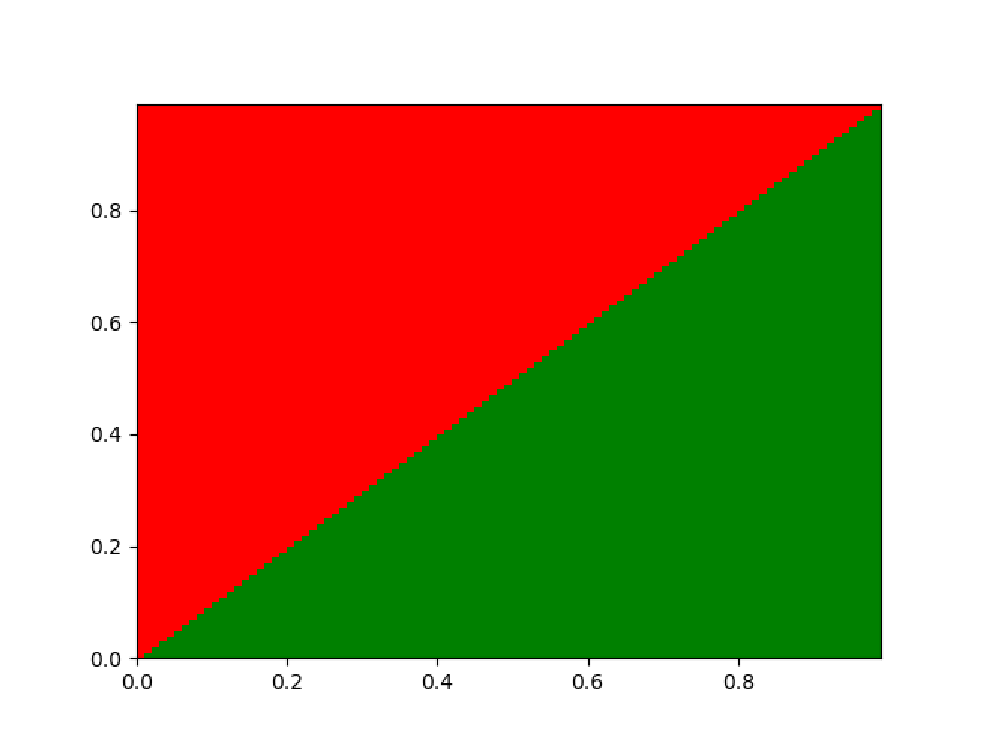
\includegraphics[width=0.5\textwidth]{sklearn_SVC.eps}\\
	This is the graph produced by the LASVM model. \\
	\includegraphics[width=0.5\textwidth]{lasvm.eps}\\
\end{enumerate}


\newpage

\subsection*{Calibration [1pt]}
Approximately how long did this homework take you to complete?
Somewhere at least 15 hours. 

\end{document}
